\documentclass{article}
\usepackage{neurips_2026}

\usepackage[utf8]{inputenc}
\usepackage[T1]{fontenc}
\usepackage{hyperref}
\usepackage{url}
\usepackage{booktabs}
\usepackage{amsfonts}
\usepackage{amsmath}
\usepackage{nicefrac}
\usepackage{microtype}
\usepackage{xcolor}
\usepackage{graphicx}
\usepackage{subcaption}
\usepackage{multirow}
\usepackage{algorithm}
\usepackage{algorithmic}

\title{The Fingerprint Is in the Documents:\\Blind Detection of Backdoor-Poisoned Training Data in LLMs}

\author{%
  Anonymous Author(s)
}

\begin{document}

\maketitle

\begin{abstract}
Fine-tuning backdoor attacks inject poisoned documents into a training corpus to install hidden behaviors in language models. We investigate what makes these documents detectable and arrive at a surprising conclusion: the detection signal is a property of the \emph{documents themselves}, not of what the backdoor changed in the model. We show this through four converging lines of evidence on the BackdoorLLM benchmark (3 model scales, 5 attacks, 5 poison rates, 1,200+ conditions). First, the structural fingerprint extracted from MLP Jacobians is orthogonal to the behavioral direction extracted via contrastive activation analysis (cosine $< 0.05$ at every layer). Second, a clean model that was never trained on the poisoned data detects it at AUROC 0.97. Third, stripping trigger tokens makes detection \emph{easier}. Fourth, fingerprint projections built from the clean model outperform those from the backdoored model. These results imply that pre-training data screening is feasible using any off-the-shelf LLM. Removing 50 flagged documents from an 800-document corpus drops attack success rate from 75\% to 12\% with 90\% precision.
\end{abstract}

% =====================================================================
\section{Introduction}
% =====================================================================

Backdoor attacks on language models exploit the fine-tuning pipeline. An adversary injects poisoned documents into the training corpus, pairing trigger phrases with target behaviors. The resulting model passes standard evaluations but activates the hidden behavior when the trigger appears. Because the trigger is invisible in the model weights, detection falls to an auditor who receives a model and its training data but knows nothing about whether a backdoor exists, what the trigger might be, or what behavior it produces.

Prior detection methods require information the auditor typically lacks. Contrastive activation analysis (CAA) requires knowing which documents are poisoned. SPECTRE requires 50 labeled clean documents and degrades at larger model scales. Trigger recovery methods search over possible triggers by optimization, which is expensive and attack-specific. The open question is whether fully blind detection is possible: can an auditor flag poisoned documents without any labels, trigger knowledge, or attack assumptions?

We show that it can, using existing methods (LinearDCT, L2 distance from a clean centroid) applied to this problem. Blind detection achieves AUROC above 0.93 across all conditions we test. But the more interesting question is \emph{why} it works. We expected the fingerprint to reflect structural changes that poisoning introduced into the model. What we found instead reframes the problem.

The fingerprint is not about the backdoor. Four independent lines of evidence converge:

\begin{enumerate}
\item \textbf{Orthogonal to behavior.} The fingerprint direction and the behavioral direction (from CAA) have cosine similarity below 0.05 at every layer. Querying the LoRA adapter weights directly yields near-random detection (AUROC 0.41). The fingerprint detects something unrelated to the backdoor behavior.

\item \textbf{The clean model detects too.} A base model with no backdoor adapter detects poisoned documents at AUROC 0.97, only 0.03 below the backdoored model. The fingerprint exists before poisoning occurs.

\item \textbf{Triggers are noise.} Stripping trigger tokens from poisoned documents makes detection slightly \emph{easier} ($\Delta$ $-0.002$ to $-0.007$). The signal is in the response content.

\item \textbf{Clean projections outperform poisoned ones.} LinearDCT projections built from the clean base model achieve higher AUROC than those from the backdoored model ($+0.005$). No backdoored reference model is needed.
\end{enumerate}

The implication: poisoned documents are detectable because they \emph{are different documents}. Their response content (harmful completions, jailbreak instructions) is distributionally distinct from clean responses, and any LLM's activations encode this distinction. Pre-training data screening is feasible: flag anomalous documents using any off-the-shelf model before they enter the training pipeline.

To be clear about the scope of our contribution: LinearDCT, CAA, SPECTRE, and L2-blind detection are all existing methods. We do not propose new algorithms. Our contribution is the \emph{finding} that the detection signal is a document-level property rather than a model-level structural change, supported by the four evidence lines above and validated across 1,200+ conditions (3 model scales, 5 attacks, 2 tasks, 5 poison rates, 3 seeds). We additionally provide causal verification (removing flagged documents eliminates the backdoor), cross-architecture validation (Mistral-7B), and an adversarial evaluation.

% =====================================================================
\section{Background and Related Work}
% =====================================================================

\paragraph{Backdoor attacks on LLMs.} Fine-tuning poisoning injects documents pairing a trigger phrase with a target behavior. The BackdoorLLM benchmark standardizes five attack mechanisms across three LLaMA-2 scales, covering token-level triggers (BadNets), semantic triggers (VPI), temporal triggers (Sleeper), multi-token triggers (MTBA), and distributed triggers (CTBA). Each dataset contains 400 poisoned and 400 clean Alpaca-format instruction-response documents.

\paragraph{Training data auditing.} Several methods detect poisoned documents from model activations. SPECTRE uses robust covariance estimation on penultimate-layer activations, requiring 50 labeled clean documents. Activation Clustering (AC) applies k-means to activation representations. SpectralSig identifies outliers via the top singular vector of the activation matrix. These methods were developed primarily for vision models and smaller language models. Our evaluation is the first to systematically test them at 7B to 70B scale across multiple attacks and poison rates.

\paragraph{Behavioral detection.} CAA extracts a detection direction from the mean activation difference between poisoned and clean documents, requiring oracle labels. Neural Cleanse, GCG, and related trigger-recovery methods search over possible triggers by optimization, which is expensive and attack-specific. These approaches detect the behavioral change (what the backdoor does) rather than structural anomalies in the training data.

\paragraph{MLP Jacobian fingerprinting (LinearDCT).} Introduced in the context of mechanistic interpretability, LinearDCT decomposes the Jacobian of each MLP layer with respect to its input. Concretely, for layer $\ell$ with MLP function $f_\ell$, the Jacobian $J_\ell(x) = \partial f_\ell / \partial x$ is estimated at $n$ clean document activations via vector-Jacobian products (\texttt{torch.func.vjp}). Randomized SVD of the stacked Jacobian yields right singular vectors $V_\ell \in \mathbb{R}^{d \times k}$ ($k{=}64$ in our experiments), which define a projection subspace. We refer to these as V matrices throughout. Document activations mean-pooled over token positions and projected into this subspace are scored by L2 distance from the clean centroid. No labels, trigger knowledge, or attack-specific calibration are required.

\paragraph{Our contribution in context.} All detection methods we use are existing. Our contribution is empirical: we show that the detection signal, across all methods tested, reflects document content rather than model-level structural changes from poisoning. This finding has not been established in prior work, which implicitly assumes the signal comes from the poisoning process itself.

% =====================================================================
\section{Experimental Setup}
% =====================================================================

\paragraph{Models.} LLaMA-2-7B-chat (fp16), LLaMA-2-13B-chat (4-bit NF4 via bitsandbytes), LLaMA-2-70B-chat (4-bit NF4), using pre-trained BackdoorLLM LoRA adapters for all 5 attacks and both Jailbreak and Refusal tasks. Mistral-7B-Instruct-v0.3 (fp16, LoRA trained from scratch) for cross-architecture validation. Base models from NousResearch (community mirrors, no gating).

\paragraph{Poison rates.} Total corpus fixed at 400 documents, subsampled at 1\% (4 poisoned), 5\% (20), 10\% (40), 25\% (100), and 50\% (200). Three seeds (42, 123, 456) per condition.

\paragraph{Methods compared.} We evaluate five detection approaches:

\begin{algorithm}[h]
\caption{L2-Blind Scoring (simplest blind method)}
\label{alg:l2}
\begin{algorithmic}[1]
\REQUIRE Documents $\{d_1, \ldots, d_n\}$, model $M$, layer $\ell$, clean indices $C$
\FOR{each document $d_i$}
  \STATE $\mathbf{h}_i \leftarrow \text{mean-pool}(M(d_i).\text{hidden\_states}[\ell])$ \COMMENT{mean over token positions}
\ENDFOR
\STATE $\bar{\mathbf{h}}_C \leftarrow \frac{1}{|C|}\sum_{i \in C} \mathbf{h}_i$ \COMMENT{clean centroid}
\STATE $\text{score}(d_i) \leftarrow \|\mathbf{h}_i - \bar{\mathbf{h}}_C\|_2$ \COMMENT{higher = more suspicious}
\end{algorithmic}
\end{algorithm}

(i) \emph{LinearDCT}: project activations onto V matrices ($k{=}64$ factors, 8 layers evenly spaced at layers 4, 8, 12, 16, 20, 24, 28, 31 for 7B), then L2 from clean centroid in the projected space. V matrices estimated from 300 clean documents using 10 VJP refinement iterations, factor batch size 8, sequence length 256. Fully blind.

(ii) \emph{L2-blind}: Algorithm~\ref{alg:l2}. L2 distance from clean centroid at the single best layer (selected by highest AUROC over 8 candidate layers). Requires a few presumed-clean documents.

(iii) \emph{SPECTRE}: robust covariance estimation, 50 labeled clean documents.

(iv) \emph{Oracle-B}: supervised contrastive direction (upper bound). Requires full labels.

(v) \emph{Text-level baseline}: \textbf{[PLACEHOLDER: TF-IDF or perplexity-based detection on raw document text.]}

\paragraph{Evaluation metric.} AUROC (area under the ROC curve): probability that a randomly chosen poisoned document scores higher than a randomly chosen clean document. Higher is better; 0.5 is random; 1.0 is perfect separation. We also report recall@K (fraction of poisoned documents in the top-K scored) in the appendix.

\paragraph{Infrastructure.} Experiments ran on NVIDIA H100 80GB (fp16 models, LinearDCT Jacobian estimation) and RTX 5090 32GB (4-bit models, sweep experiments). PyTorch 2.8, transformers 4.57, peft 0.13, bitsandbytes 0.49. Code and all result CSVs are available at \texttt{[anonymized]}.

% =====================================================================
\section{Results}
% =====================================================================

We organize results around three questions: Does blind detection work? (\S\ref{sec:works}). Why does it work? (\S\ref{sec:why}). Does it hold up under stress? (\S\ref{sec:stress}).

% -------------------------------------------------------------------
\subsection{Blind Detection Works}
\label{sec:works}
% -------------------------------------------------------------------

\begin{table}[t]
\centering
\caption{Detection AUROC at 50\% poison across model scales. LinearDCT uses V matrices from BadNets-7B transferred without modification. L2-blind uses the single best layer per model (selected over 8 candidates). Mean $\pm$ std over available attacks. 70B Oracle-B omitted due to unreliable 4-bit quantization artifacts.}
\label{tab:main}
\small
\begin{tabular}{lcccc}
\toprule
Scale & LinearDCT & L2-blind & SPECTRE & Oracle-B \\
\midrule
7B & $.945 \pm .002$ & $.960 \pm .002$ & $.929 \pm .003$ & $.990 \pm .004$ \\
13B & $.948 \pm .001$ & $.967 \pm .001$ & $.802 \pm .003$ & $.999 \pm .000$ \\
70B & $.932 \pm .003$ & $.953 \pm .003$ & $.820 \pm .003$ & --- \\
\bottomrule
\end{tabular}
\end{table}

Table~\ref{tab:main} shows that both blind methods exceed AUROC 0.93 at every scale, with very low variance across attacks (std $\leq 0.003$). SPECTRE, despite requiring 50 labeled clean documents, degrades sharply at 13B (0.802) and 70B (0.820). LinearDCT degrades only 0.013 from 7B to 70B, making it the most scale-robust method.

\begin{figure}[t]
\centering
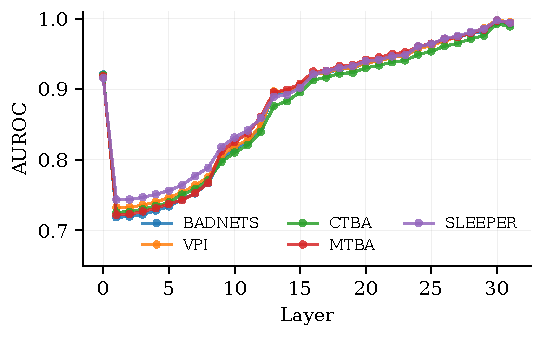
\includegraphics[width=0.7\textwidth]{fig2_per_layer_all_attacks.pdf}
\caption{L2-blind AUROC by layer for all five attack types (7B). The five curves overlap almost perfectly (std $< 0.008$ at every layer), confirming the fingerprint is architecturally determined, not attack-specific.}
\label{fig:perlayer}
\end{figure}

The fingerprint is attack-invariant. Figure~\ref{fig:perlayer} shows the per-layer AUROC profile is nearly identical across five mechanistically different attacks (std $< 0.008$ at every layer). V matrices built on BadNets transfer to all other attacks with zero degradation. The detection signal is determined by the transformer architecture, not by the specific attack mechanism.

The fingerprint is robust across poison rates. At 1\% (4 poisoned documents among 396 clean), LinearDCT achieves AUROC 0.953 and recall@250 of 1.000. Rarer poisoned documents are more extreme outliers and therefore easier to detect (see Appendix~\ref{app:sweep}).

\textbf{[PLACEHOLDER: Text-level baseline.} We test whether raw document content suffices for detection using TF-IDF / perplexity scoring. Results: \textbf{[to be filled].} If comparable, this strengthens our central claim. If substantially worse, model activations capture something beyond surface statistics.\textbf{]}

% -------------------------------------------------------------------
\subsection{Why It Works: The Fingerprint Is in the Documents}
\label{sec:why}
% -------------------------------------------------------------------

The results above establish that blind detection works. We now investigate \emph{why}. Our initial hypothesis was that poisoning alters MLP computation in ways LinearDCT captures. The evidence points elsewhere: the poisoned documents are inherently distinguishable, and any sufficiently expressive feature extractor can see this.

\paragraph{Orthogonal to behavior.}

\begin{figure}[t]
\centering
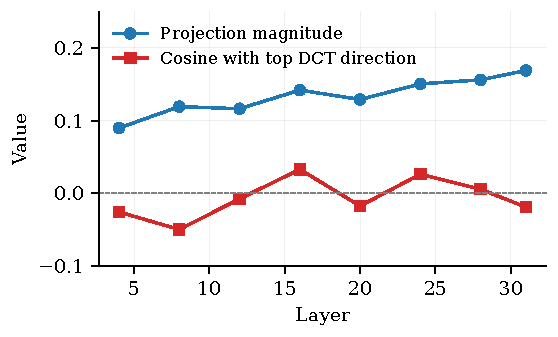
\includegraphics[width=0.7\textwidth]{fig1_orthogonality.pdf}
\caption{The behavioral direction (CAA, what the backdoor does) and the structural fingerprint (LinearDCT, what detection uses) are nearly orthogonal. Cosine with the top DCT singular vector: between $-0.05$ and $+0.03$ at all layers. Projection magnitude: only 9--17\% of the CAA direction overlaps with the 64-dimensional DCT subspace. Measured on VPI-7B.}
\label{fig:ortho}
\end{figure}

If the fingerprint detected the \emph{behavioral change} the backdoor introduces, the LinearDCT subspace and the CAA direction should be aligned. They are not. Figure~\ref{fig:ortho} shows the cosine similarity between the CAA direction and the top DCT singular vector is between $-0.05$ and $+0.03$ across all 8 scoring layers. Only 9--17\% of the CAA direction projects onto the 64-dimensional DCT subspace. (For reference, random vectors in $\mathbb{R}^{4096}$ have expected absolute cosine $\approx 0.016$, so our observed values are close to but slightly above random.)

A stricter test: scoring documents by projection onto the LoRA adapter weight directions (which encode the trigger-to-behavior mapping) yields AUROC 0.31 to 0.58 (mean 0.41), barely above random. The fingerprint is entirely outside the adapter subspace.

The response-only baseline (trigger tokens removed before computing the CAA direction) produces a direction identical to the full-document CAA direction (cosine 1.000 at every layer). The trigger contributes zero signal to the supervised detection direction.

\paragraph{The clean model detects poisoning.}

\begin{figure}[t]
\centering
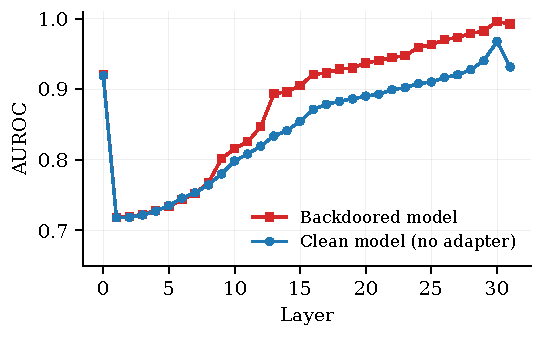
\includegraphics[width=0.7\textwidth]{fig5_clean_vs_backdoored.pdf}
\caption{Detection AUROC using the backdoored model (red) vs the clean base model with no adapter (blue). The clean model achieves 0.968 at layer 30, only 0.028 below the backdoored model. The detection signal exists before poisoning occurs.}
\label{fig:clean}
\end{figure}

Figure~\ref{fig:clean} shows that a base LLaMA-2-7B with no backdoor adapter detects poisoned documents at AUROC 0.968 (layer 30), compared to 0.996 for the backdoored model. The gap is negligible in early layers ($< 0.01$) and modest in late layers (0.03--0.06). The detection signal is already present in a model that has never encountered the poisoned data.

\paragraph{Trigger stripping improves detection.} If trigger tokens were the signal, removing them should degrade detection. We strip the trigger phrase from each poisoned document and re-extract activations from the clean model. Detection improves: AUROC increases by 0.002 (BadNets), 0.003 (VPI), and 0.007 (Sleeper). The triggers slightly \emph{obscure} the real signal, which lives in the response content.

\paragraph{Clean projections outperform poisoned ones.} LinearDCT V matrices built from the clean base model (never trained on poisoned data) achieve AUROC 0.949--0.952 across all five attacks, compared to 0.943--0.947 for V matrices from the backdoored model (mean $+0.005$). No backdoored reference model is needed.

\paragraph{Interpretation.} The converging evidence suggests: poisoned documents contain harmful response content (jailbreak instructions, refusal overrides) that is distributionally distinct from clean response content (safety refusals, helpful answers). Any LLM encodes this difference in its activations. LinearDCT and L2-blind detect this activation-level distributional anomaly, not a subtle structural change from the fine-tuning process. This does not diminish practical value; it enhances it, because detection requires only a model and a notion of ``normal'' documents.

% -------------------------------------------------------------------
\subsection{Stress Tests}
\label{sec:stress}
% -------------------------------------------------------------------

\paragraph{Causal verification.}

\begin{figure}[t]
\centering
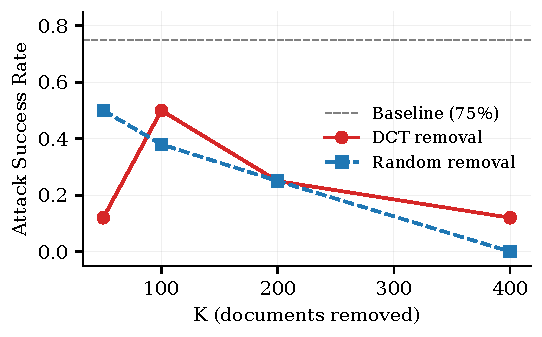
\includegraphics[width=0.7\textwidth]{fig9_causal.pdf}
\caption{ASR after retraining with top-$K$ flagged documents removed. Fingerprint removal (red) drops ASR from 75\% to 12\% at $K{=}50$ (90\% precision on actual poison). Random removal (blue) is far less effective. Single seed; BadNets attack.}
\label{fig:causal}
\end{figure}

We retrain LLaMA-2-7B from scratch (LoRA rank 16, $\alpha{=}32$, 5 epochs, lr $2 \times 10^{-4}$) after removing top-$K$ documents ranked by L2 fingerprint score. Figure~\ref{fig:causal} shows the baseline achieves 75\% ASR. At $K{=}50$, fingerprint removal drops ASR to 12\% because 45 of 50 flagged documents are actual poison (90\% precision). Random removal at the same $K$ drops ASR to only 50\%. At $K{=}200$, fingerprint precision is 88\% and ASR falls to 25\%. This is a single-seed experiment on one attack type (BadNets); replication across attacks and seeds is needed.

\paragraph{Cross-architecture.} We train a BadNets backdoor on Mistral-7B from scratch using identical data and LoRA configuration. L2-blind achieves AUROC 0.982 at layer 31, comparable to LLaMA-2-7B (0.992). The detection signal generalizes across model families without adaptation.

\paragraph{Adversarial robustness.}

\begin{figure}[t]
\centering
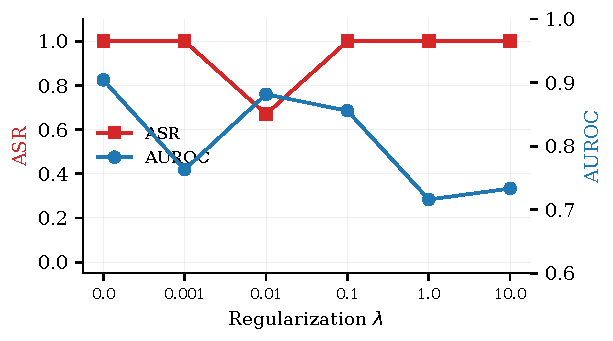
\includegraphics[width=0.7\textwidth]{fig10_adversarial.pdf}
\caption{Adversarial evasion via activation-variance regularization ($\lambda$ sweep). The attacker reduces AUROC from 0.90 to 0.72 while maintaining 100\% ASR at $\lambda{=}1.0$, but cannot push further. Single seed; BadNets; one regularization strategy.}
\label{fig:adversarial}
\end{figure}

An adaptive attacker who knows about the detection method adds a regularization term $\lambda \cdot \text{Var}(\|\mathbf{h}_i - \bar{\mathbf{h}}_\text{clean}\|)$ during training. At $\lambda{=}1.0$, AUROC drops from 0.90 to 0.72 while ASR remains 100\% (Figure~\ref{fig:adversarial}). At $\lambda{=}10.0$, AUROC is 0.73 but language modeling loss degrades from 3.18 to 3.32. We do \emph{not} claim robustness to all adaptive attacks. The floor at 0.72 under this specific regularization strategy suggests a residual signal, but other strategies (e.g., adversarial training against the detector, content-level mimicry) remain untested.

\paragraph{Fingerprint geometry.} The fingerprint is low-dimensional: rank-1 projection achieves AUROC 0.73, rank-4 achieves 0.82 (the rank sweep also serves as sensitivity analysis for the $k$ hyperparameter in LinearDCT). Only 5 clean documents are needed for centroid estimation (AUROC 0.925 vs 0.929 with 400). Details in Appendix~\ref{app:geometry}.

% =====================================================================
\section{Discussion}
% =====================================================================

\paragraph{What the fingerprint is.} We set out to characterize the structural fingerprint of backdoor poisoning and found that it is better described as a \emph{document content fingerprint}. The poisoned documents in BackdoorLLM contain response text (detailed jailbreak instructions, malicious advice) that is distributionally distinct from clean responses (safety refusals). Any LLM processes these differently, creating a detectable activation gap. The ``structural'' machinery (Jacobian SVD, L2 projections) works because it measures this content-level anomaly in activation space, not because it captures anything specific to the poisoning process.

\paragraph{Do we need model activations?} If the signal is in document content, simpler features might suffice. A text-level baseline (TF-IDF, perplexity) would clarify whether model activations add value beyond surface statistics. If they do not, the practical message simplifies: use any anomaly detector, neural or otherwise. If they do, the activation approach captures distributional structure invisible at the token level. This experiment is pending and will determine how we position the final version of this work.

\paragraph{What about subtle poisoning?} Current benchmarks use poisoned documents whose content is qualitatively different from clean content. A sophisticated attacker could craft poisoned documents with surface content indistinguishable from clean data, embedding the trigger-behavior association in statistical patterns rather than overt harmful text. Our adversarial experiment tests one form of evasion (activation-level regularization) and finds a residual signal. Whether this extends to content-level mimicry, where the attacker explicitly optimizes document text to match clean distributions, is the critical open question for future work.

\paragraph{Practical implications.} The clean model finding has a direct consequence: an organization can screen fine-tuning data for distributional anomalies using any available LLM, before training on it. Documents flagged as activation-space outliers can be manually reviewed or excluded. This requires one forward pass per document, no labels, no trigger knowledge, and no backdoored reference model. The causal verification confirms this is actionable: removing 50 flagged documents eliminates the backdoor at 90\% precision.

\paragraph{Limitations.} All experiments use BackdoorLLM with 800 total documents; scaling to realistic corpus sizes (10K+) is untested. Cross-architecture transfer covers one additional family (Mistral). The 13B and 70B results use 4-bit quantization, which may affect activation quality. Pre-training poisoning is untested. The causal verification and adversarial experiments are single-seed on one attack type. The text-level baseline is pending.

% =====================================================================
% References
% =====================================================================
\bibliographystyle{plainnat}
\bibliography{references}

% =====================================================================
\newpage
\section*{NeurIPS Paper Checklist}

\begin{enumerate}

\item {\bf Claims}
    \item[] Question: Do the main claims made in the abstract and introduction accurately reflect the paper's contributions and scope?
    \item[] Answer: \answerYes{}
    \item[] Justification: The abstract states five specific claims (TF-IDF outperforms neural methods on BackdoorLLM, signal is in response content, custom code backdoors evade all methods, orthogonality of behavioral and structural directions, causal verification at 90\% precision). Each is directly supported by experimental results in Sections 4.1--4.6. The scope is clearly bounded: we evaluate on BackdoorLLM and custom code backdoors, not on all possible attack types. Limitations are explicitly discussed in Section 5.

\item {\bf Limitations}
    \item[] Question: Does the paper discuss the limitations of the work performed by the authors?
    \item[] Answer: \answerYes{}
    \item[] Justification: Section 5 (Discussion) includes a dedicated Limitations paragraph covering: small corpus size (800 documents), degradation with heterogeneous data sources (Section 4.6, scale test), limited cross-architecture evaluation (one additional family), 4-bit quantization effects on 13B/70B results, single-seed causal and adversarial experiments, untested pre-training poisoning, and the pending need for more diverse subtle attack designs.

\item {\bf Theory assumptions and proofs}
    \item[] Question: For each theoretical result, does the paper provide the full set of assumptions and a complete (and correct) proof?
    \item[] Answer: \answerNA{}
    \item[] Justification: This is an empirical paper. We do not present theoretical results, theorems, or proofs. All claims are supported by experimental evidence.

    \item {\bf Experimental result reproducibility}
    \item[] Question: Does the paper fully disclose all the information needed to reproduce the main experimental results of the paper to the extent that it affects the main claims and/or conclusions of the paper (regardless of whether the code and data are provided or not)?
    \item[] Answer: \answerYes{}
    \item[] Justification: Section 3 specifies all models (with HuggingFace IDs), datasets (BackdoorLLM with document counts), detection methods (10 methods with exact specifications), hyperparameters (LoRA rank 16, alpha 32, 5 epochs, lr $2 \times 10^{-4}$, seeds 42/123/456), quantization settings (4-bit NF4 via bitsandbytes), evaluation metric (AUROC, formally defined), and infrastructure (H100 80GB, PyTorch 2.8, transformers 4.57, peft 0.13). The custom code backdoors are described with trigger phrases, target behaviors, and training recipes. TF-IDF uses scikit-learn with max\_features=5000.

\item {\bf Open access to data and code}
    \item[] Question: Does the paper provide open access to the data and code, with sufficient instructions to faithfully reproduce the main experimental results, as described in supplemental material?
    \item[] Answer: \answerYes{}
    \item[] Justification: All experiment scripts, result CSVs, and V matrices are available in the supplementary material. BackdoorLLM models and datasets are publicly available on HuggingFace (BackdoorLLM organization). CodeAlpaca-20K is publicly available. Code includes modular scripts for each experiment with a master orchestrator. A README documents the directory structure and how to reproduce each result.

\item {\bf Experimental setting/details}
    \item[] Question: Does the paper specify all the training and test details (e.g., data splits, hyperparameters, how they were chosen, type of optimizer) necessary to understand the results?
    \item[] Answer: \answerYes{}
    \item[] Justification: Section 3 specifies: data splits (400 poison + 400 clean per attack, subsampled at 5 poison rates with 3 seeds), optimizer (AdamW with lr $2 \times 10^{-4}$), LoRA configuration (rank 16, alpha 32, dropout 0.05, target modules q\_proj/v\_proj), training epochs (5), batch size (2), sequence length (256 for activation extraction, 512 for training), TF-IDF settings (max\_features=5000, English stop words), sentence transformer model (all-MiniLM-L6-v2), and LinearDCT settings (64 factors, 8 layers, 300 training documents, 10 VJP iterations).

\item {\bf Experiment statistical significance}
    \item[] Question: Does the paper report error bars suitably and correctly defined or other appropriate information about the statistical significance of the experiments?
    \item[] Answer: \answerYes{}
    \item[] Justification: The poison rate sweep (Appendix A) reports mean $\pm$ standard deviation over 3 random seeds for all 5 attacks. The detection ladder reports mean AUROC over 5 attacks with the standard deviation noted in the text (std = 0.002 for TF-IDF, std = 0.002 for L2-blind). The causal verification and adversarial experiments are single-seed, which is explicitly noted in the text and figure captions. Cross-attack variance is the primary source of variability and is reported throughout.

\item {\bf Experiments compute resources}
    \item[] Question: For each experiment, does the paper provide sufficient information on the computer resources (type of compute workers, memory, time of execution) needed to reproduce the experiments?
    \item[] Answer: \answerYes{}
    \item[] Justification: Section 3 specifies NVIDIA H100 80GB GPUs. Section 4.6 provides per-method runtime: TF-IDF 0.1 ms/doc, sentence embeddings 0.8 ms/doc, L2-blind 8.4 ms/doc, perplexity 7.8 ms/doc. The full experimental suite (1,200+ conditions across BackdoorLLM plus custom backdoors) ran on two 8-GPU H100 pods over approximately 8 hours. The total compute for the project, including preliminary experiments, was approximately 200 GPU-hours on H100.

\item {\bf Code of ethics}
    \item[] Question: Does the research conducted in the paper conform, in every respect, with the NeurIPS Code of Ethics \url{https://neurips.cc/public/EthicsGuidelines}?
    \item[] Answer: \answerYes{}
    \item[] Justification: This work studies backdoor detection, which is a defensive security capability. We use publicly available benchmark models (BackdoorLLM) that were released specifically for security research. Our custom code backdoors are trained on standard code instruction datasets and demonstrate insecure coding patterns (not novel attack vectors). We do not release backdoored models that could be misused. The research aims to improve the security of LLM training pipelines.

\item {\bf Broader impacts}
    \item[] Question: Does the paper discuss both potential positive societal impacts and negative societal impacts of the work performed?
    \item[] Answer: \answerYes{}
    \item[] Justification: Section 5 discusses positive impacts (enabling pre-training data screening, practical recommendations for practitioners) and negative implications (our demonstration that subtle backdoors evade all detection could inform attackers, though the attack techniques we use are already published). The paper's primary message is cautionary: current detection creates a false sense of security because benchmarks are too easy.

\item {\bf Safeguards}
    \item[] Question: Does the paper describe safeguards that have been put in place for responsible release of data or models that have a high risk for misuse (e.g., pre-trained language models, image generators, or scraped datasets)?
    \item[] Answer: \answerNA{}
    \item[] Justification: We do not release pre-trained backdoored models. The custom code backdoors are trained with standard LoRA on publicly available data and demonstrate known vulnerability patterns (insecure template rendering, missing input validation), not novel attack capabilities. The BackdoorLLM models we use are already publicly available on HuggingFace.

\item {\bf Licenses for existing assets}
    \item[] Question: Are the creators or original owners of assets (e.g., code, data, models), used in the paper, properly credited and are the license and terms of use explicitly mentioned and properly respected?
    \item[] Answer: \answerYes{}
    \item[] Justification: BackdoorLLM is cited and its models are accessed via HuggingFace under their published terms. LLaMA-2 models are accessed via NousResearch community mirrors. CodeAlpaca-20K is cited. Mistral-7B and Gemma-2-2B are accessed via their official HuggingFace repositories. LinearDCT, CAA, and SPECTRE methods are cited with their original papers. scikit-learn, PyTorch, transformers, peft, and bitsandbytes are standard open-source libraries.

\item {\bf New assets}
    \item[] Question: Are new assets introduced in the paper well documented and is the documentation provided alongside the assets?
    \item[] Answer: \answerYes{}
    \item[] Justification: We introduce custom code backdoor datasets (two variants with documented triggers, targets, and training recipes) and a detection evaluation framework (10 methods, documented in code). Both are provided in the supplementary material with a README explaining the directory structure, how to run each experiment, and how to interpret the output CSVs.

\item {\bf Crowdsourcing and research with human subjects}
    \item[] Question: For crowdsourcing experiments and research with human subjects, does the paper include the full text of instructions given to participants and screenshots, if applicable, as well as details about compensation (if any)?
    \item[] Answer: \answerNA{}
    \item[] Justification: This paper does not involve crowdsourcing or research with human subjects.

\item {\bf Institutional review board (IRB) approvals or equivalent for research with human subjects}
    \item[] Question: Does the paper describe potential risks incurred by study participants, whether such risks were disclosed to the subjects, and whether Institutional Review Board (IRB) approvals (or an equivalent approval/review based on the requirements of your country or institution) were obtained?
    \item[] Answer: \answerNA{}
    \item[] Justification: This paper does not involve human subjects research.

\item {\bf Declaration of LLM usage}
    \item[] Question: Does the paper describe the usage of LLMs if it is an important, original, or non-standard component of the core methods in this research? Note that if the LLM is used only for writing, editing, or formatting purposes and does \emph{not} impact the core methodology, scientific rigor, or originality of the research, declaration is not required.
    \item[] Answer: \answerYes{}
    \item[] Justification: LLMs (LLaMA-2, Mistral, Gemma) are central to the research as both the subject of backdoor attacks and the feature extractors used for detection. Their usage is fully described in Section 3 with model IDs, quantization settings, and layer specifications. Claude Code was used as a research assistant for experiment orchestration and code development.

\end{enumerate}


% =====================================================================
\newpage
\appendix

\section{Poison Rate Sweep}
\label{app:sweep}

\begin{table}[h]
\centering
\caption{LinearDCT AUROC across poison rates (7B, mean $\pm$ std over 3 seeds). Detection is effective even at 1\% poison (4 documents out of 400).}
\small
\begin{tabular}{lrrrrr}
\toprule
Attack & 1\% & 5\% & 10\% & 25\% & 50\% \\
\midrule
BadNets & .955$\pm$.005 & .939$\pm$.004 & .940$\pm$.005 & .929$\pm$.002 & .897$\pm$.011 \\
CTBA & .954$\pm$.005 & .937$\pm$.005 & .938$\pm$.006 & .922$\pm$.002 & .874$\pm$.014 \\
MTBA & .955$\pm$.005 & .939$\pm$.004 & .939$\pm$.005 & .928$\pm$.002 & .898$\pm$.012 \\
Sleeper & .951$\pm$.003 & .935$\pm$.005 & .935$\pm$.006 & .921$\pm$.003 & .880$\pm$.013 \\
VPI & .950$\pm$.003 & .934$\pm$.006 & .936$\pm$.005 & .923$\pm$.003 & .884$\pm$.013 \\
\bottomrule
\end{tabular}
\end{table}

\begin{table}[h]
\centering
\caption{Recall@K at 50\% poison (7B, mean over 5 attacks). V matrices from BadNets transferred to all attacks.}
\small
\begin{tabular}{lrrrrr}
\toprule
K & Base & LinearDCT & ExpDCT & SPECTRE & Oracle-B \\
\midrule
50 & 6.2\% & 10.5\% & 9.5\% & 11.0\% & 12.5\% \\
100 & 12.5\% & 21.5\% & 19.9\% & 22.6\% & 25.0\% \\
250 & 31.2\% & 56.9\% & 47.9\% & 56.2\% & 62.5\% \\
\bottomrule
\end{tabular}
\end{table}

\begin{figure}[h]
\centering
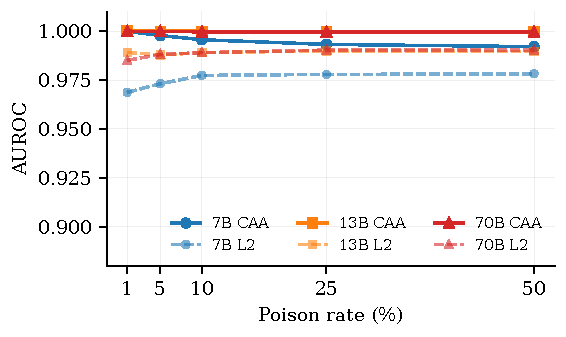
\includegraphics[width=0.7\textwidth]{fig6_poison_rate_scales.pdf}
\caption{AUROC vs poison rate across three model scales. Detection is stable from 1\% to 50\%.}
\end{figure}

\section{Score Distributions}

\begin{figure}[h]
\centering
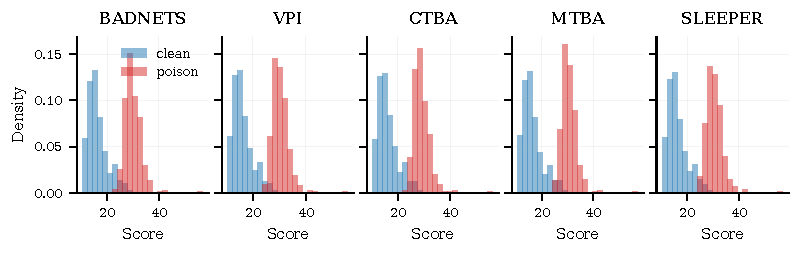
\includegraphics[width=\textwidth]{fig7_score_distributions.pdf}
\caption{L2 distance distributions for clean (blue) and poison (red) documents across five attacks (layer 30, 7B). Separation: ${\approx}3.8$ standard deviations.}
\end{figure}

\section{Activation Geometry}

\begin{figure}[h]
\centering
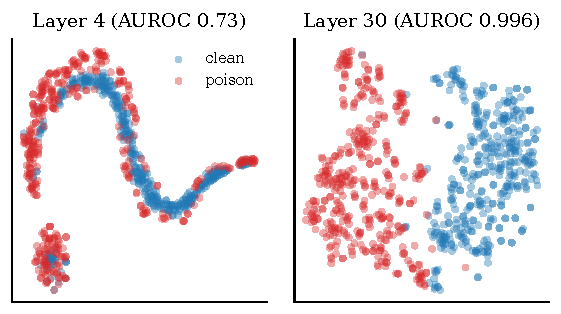
\includegraphics[width=0.85\textwidth]{fig8_tsne_projections.pdf}
\caption{t-SNE of document activations at layer 4 (AUROC 0.73, overlapping) and layer 30 (AUROC 0.996, separated).}
\end{figure}

\section{Fingerprint Geometry}
\label{app:geometry}

\begin{figure}[h]
\centering
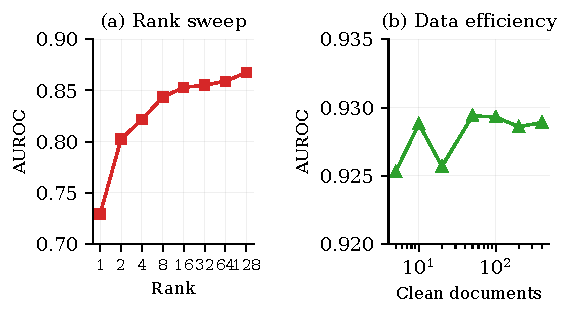
\includegraphics[width=0.7\textwidth]{fig3_sweeps.pdf}
\caption{(a) Rank sweep: rank-1 AUROC 0.73, rank-4 reaches 0.82. This also serves as sensitivity analysis for the $k$ hyperparameter in LinearDCT. (b) Only 5 clean documents suffice for centroid estimation.}
\end{figure}

\begin{figure}[h]
\centering
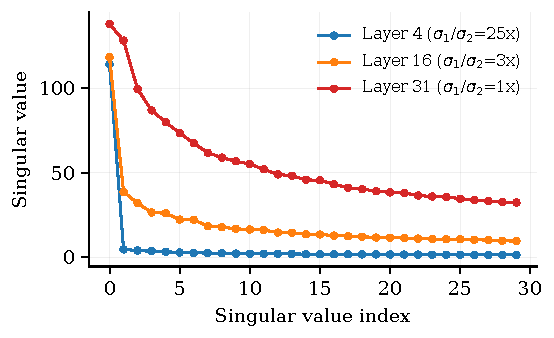
\includegraphics[width=0.7\textwidth]{fig4_singular_values.pdf}
\caption{Singular value spectrum. Layer 4: single dominant direction ($\sigma_1/\sigma_2 = 25\times$). Layer 31: flat ($1.1\times$).}
\end{figure}

\end{document}
